\section{Casos de Uso Principais}

\subsection{Identificação}

Para utilizar o programa o utilizador deve compilá-lo. Para isso deve executar o comando "make". Se o código já tiver sido previamente compilado deve ser executado "make clean".

Para transmitir um ficheiro o utilizador deve possuir dois terminais ligados por uma porta série.
\begin{itemize}
    \item Comando a executar no terminal do transmissor - ./rcompy -t -s \textit{caminho para a porta série} -f \textit{caminho para o ficheiro}
    \item Comando a executar no terminal do recetor - ./rcompy -r -s \textit{caminho para a porta série} -f \textit{caminho para o novo ficheiro}
    \item Opções extra como -x \textit{frequência de erros nos dados} ou -z \textit{frequência de erros no cabeçalho} e -p \textit{tempo de propagação} podem ser acrescentadas ao recetor para simulação de erros e tempo de propagação
    \item Para transmitir um ficheiro o utilizador deve possuir dois terminais ligados por uma porta série. 
\end{itemize}



\subsection{Sequência de Chamadas}

A sequência de chamada a funções de cada componente da aplicação é apresentada nos seguintes diagramas.

\begin{figure}[h!]
    \centering
    \begin{subfigure}{.5\textwidth}
        \centering
        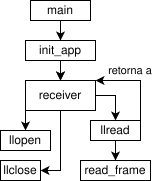
\includegraphics[width=.5\linewidth]{img/EsquemaChamadaAFuncoesReceiver.png}
        \caption{Esquema de Chamadas do Recetor}
    \end{subfigure}%
    \begin{subfigure}{.5\textwidth}
        \centering
        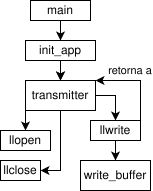
\includegraphics[width=.5\linewidth]{img/EsquemaChamadaAFuncoesTransmiter.png}
        \caption{Esquema de Chamadas do Transmissor}
    \end{subfigure}
    \caption{Esquema de Chamadas do Programa}
\end{figure}

Apenas foram apresentadas as funções mais importantes, o fluxo completo pode ser obtido analisando o código e os seus comentários.


